\documentclass[12pt]{article}
\usepackage{graphics}
\usepackage[top=1in,bottom=1in,left=1in,right=1in]{geometry}
\usepackage{alltt}
\usepackage{array}	
\usepackage{graphicx}
\usepackage{tabularx}
\usepackage{verbatim}
\usepackage{setspace}
\usepackage{listings}

\usepackage{amssymb,amsmath, amsthm}
\usepackage{zed-csp}
\usepackage[cc]{titlepic}

\title{COMP 335: Introduction to Theoretical Computer Science\\
\ \\
Assignment 1}
\author{Nathan Grenier}
\date{\today \\ Fall 2024}

\begin{spacing}{1.5}
\begin{document}
\maketitle

\newpage

\begin{enumerate}

\item[1.] [15 Points] For each of the following statements write if the statement is TRUE or FALSE. If the statement is TRUE then provide a proof. If the statement is FALSE then provide a counter-example.

\begin{enumerate}
	
	\item For every language $L$ we have $L^2 \subseteq L^3$
	
	\noindent \textbf{Answer:}

	\noindent \textbf{Proof:} 
	
	\item For every two languages $L_1$ and $L_2$ we have $(L_1 \cup L_2)^* \subseteq (L_1L_2)^*$
	
	\noindent \textbf{Answer:}

	\noindent \textbf{Proof:} 

	\item Let $L_1$ and $L_2$ be two languages such that $\lambda \in L_1 \cap L_2$. Then it holds that $(L_1L_2)^* = (L_2L_1)^*$
	
	\noindent \textbf{Answer:}

	\noindent \textbf{Proof:} 
	
\end{enumerate}

\newpage

\item[2.] [10 Points] The following is a transition diagram for a DFA over the alphabet $\Sigma = \{0,1\}$. Answer the following questions about this automaton:

\begin{figure}[h!]
	\centering
	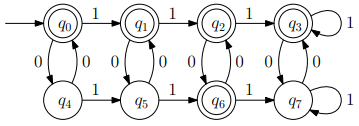
\includegraphics[width=0.6\textwidth]{img/q2_automata.png}
\end{figure}

\begin{enumerate}
	\item What is the start state? What is the set of accept states?
	
	\noindent \textbf{Answer:}

	\item What is the sequence of states the DFA goes through on input 101100?
	
	\noindent \textbf{Answer:}

	\item Does the machine accept every string $w$ that contains exactly two 1s? Why or why not?
	
	\noindent \textbf{Answer:}

	\item Does the machine reject every string $w$ that has odd number of 0s? Why or why not?
	
	\noindent \textbf{Answer:}

	\item Describe the language accepted by the machine using the set builder notation.
	
	\noindent \textbf{Answer:}

\end{enumerate}

\newpage

\item[3.] [30 Points] For each of the following languages, give a DFA that accepts it.

\begin{enumerate}
	\item $\{ba^nb^m : n \geq 3, m \geq 2 \}$
	
	\noindent \textbf{Answer:}
	
	\item $\{w \in \{a,b \}^* : \text{every maximal substring } w \text{ consisting entirely of symbols } a \\ \text{ is of length exactly 3} \}$
		
	\noindent \textbf{Answer:}

	\item $\{w \in \{a,b \}^* : \text{$w$ does not contain $bab$ as a substring} \}$
	
	\noindent \textbf{Answer:}

	\item $\{w \in \{a,b \}^* : \text{$w$ begins with bb and $n_b(w)$ mod 3 = 0} \}$
	
	\noindent \textbf{Answer:}

	\item $\{a^mb^n : mn > 4\}$
	
	\noindent \textbf{Answer:}

	\item $\{vwv^R : v,m \in \{a,b \}^* \text{ and} |v| = 2 \}$
	
	\noindent \textbf{Answer:}
\end{enumerate}

\end{enumerate}

\end{spacing}

\end{document}